\documentclass[12pt]{article}\usepackage[]{graphicx}\usepackage[]{color}
% maxwidth is the original width if it is less than linewidth
% otherwise use linewidth (to make sure the graphics do not exceed the margin)
\makeatletter
\def\maxwidth{ %
  \ifdim\Gin@nat@width>\linewidth
    \linewidth
  \else
    \Gin@nat@width
  \fi
}
\makeatother

\definecolor{fgcolor}{rgb}{0.345, 0.345, 0.345}
\newcommand{\hlnum}[1]{\textcolor[rgb]{0.686,0.059,0.569}{#1}}%
\newcommand{\hlstr}[1]{\textcolor[rgb]{0.192,0.494,0.8}{#1}}%
\newcommand{\hlcom}[1]{\textcolor[rgb]{0.678,0.584,0.686}{\textit{#1}}}%
\newcommand{\hlopt}[1]{\textcolor[rgb]{0,0,0}{#1}}%
\newcommand{\hlstd}[1]{\textcolor[rgb]{0.345,0.345,0.345}{#1}}%
\newcommand{\hlkwa}[1]{\textcolor[rgb]{0.161,0.373,0.58}{\textbf{#1}}}%
\newcommand{\hlkwb}[1]{\textcolor[rgb]{0.69,0.353,0.396}{#1}}%
\newcommand{\hlkwc}[1]{\textcolor[rgb]{0.333,0.667,0.333}{#1}}%
\newcommand{\hlkwd}[1]{\textcolor[rgb]{0.737,0.353,0.396}{\textbf{#1}}}%
\let\hlipl\hlkwb

\usepackage{framed}
\makeatletter
\newenvironment{kframe}{%
 \def\at@end@of@kframe{}%
 \ifinner\ifhmode%
  \def\at@end@of@kframe{\end{minipage}}%
  \begin{minipage}{\columnwidth}%
 \fi\fi%
 \def\FrameCommand##1{\hskip\@totalleftmargin \hskip-\fboxsep
 \colorbox{shadecolor}{##1}\hskip-\fboxsep
     % There is no \\@totalrightmargin, so:
     \hskip-\linewidth \hskip-\@totalleftmargin \hskip\columnwidth}%
 \MakeFramed {\advance\hsize-\width
   \@totalleftmargin\z@ \linewidth\hsize
   \@setminipage}}%
 {\par\unskip\endMakeFramed%
 \at@end@of@kframe}
\makeatother

\definecolor{shadecolor}{rgb}{.97, .97, .97}
\definecolor{messagecolor}{rgb}{0, 0, 0}
\definecolor{warningcolor}{rgb}{1, 0, 1}
\definecolor{errorcolor}{rgb}{1, 0, 0}
\newenvironment{knitrout}{}{} % an empty environment to be redefined in TeX

\usepackage{alltt}
\usepackage[top=1.00in, bottom=1.0in, left=1.1in, right=1.1in]{geometry}
\renewcommand{\baselinestretch}{1.1}
\usepackage{graphicx}
\usepackage{natbib}
\usepackage{amsmath}
\bibliographystyle{..//refs/styles/besjournals.bst}
\def\labelitemi{--}
\parindent=24pt
\title{Suppliment: Reconciling historic hypotheses regarding flower-leaf sequences in temperate forests for fundamental and global change biology}
\IfFileExists{upquote.sty}{\usepackage{upquote}}{}
\begin{document}
\maketitle
\subsection*{Methods}
\subsubsection*{Climate Change and FLS:}
To evaluate how FLS patterns have overtime in association with climate change we obtained phenological data for three European woody plant species with long term records of both flower (BBCH 60) and leafout phenology (BBCH 11) from the Pan European Phenological Database \citep{PEP725}. We restricted the data set to include only stations with great than 50 years worth of data. For each species, we modeled FLS offset (day of year leafing- day of year flowering) as a function of time, using a hinge model with 1980 as break point in accordance with climate change models of \citet(). For each species, we displayed the pre-1980 mean and standard devation of FLS offset and the post-1980 change in mean FLS offset that can be associated with climate change.
\subsubsection*{Case studies}
\indent\indent \textbf{MTSV and USFS:} For these two, categorical, species level case studies, we converted verbal descriptions of flower-leaf sequences into a binary response variable. For our more inclusive "functional" definition of hysteranthy, we included species entries with descriptions \textit{"flowers before the leaves"}, \textit{"flowers before or with leaves"} and textit{"flowers with leaves"} as hysteranthous. Our more restrictive "physiological" hysteranthy definition only included species described as \textit{"flowers before the leaves"} as hysteranthous.\\
\ident For modeling trait associates we chose three predictors to represent the three major FLS hypothesis; pollination syndrome, average flowering time and minimum precipitation levels across the species range. Pollination syndrome and average flowering time we obtained directly from the data sources, and estimates of minimum precipitation came from the USDA/NRCS Conservation plants characteristics \citep{}. We coded pollination syndrome as binary, biotic or wind pollinated, with known ambophilous species in the genus \textit{Salix} assigned to the ancestral, biotic pollinated, state of angiosperms. Flowering time was the average of the range of months reported in each data source.\\
\indent \textbf{HF:} For each species in the HF data set, we calculated a continuous mean off FLS "offset" defined here as the average foliate day of the year - average floral day of the year. We approximated our "physiological" FLS characterization be defining offset as (day of leaf budburst-day of flower bud burst) and our "functional" FLS categorization by defining offset as (day of leaf expansion to 75\% of final size- day of first flower open). We also recoded the HF continuous offset variables as continuous with positive offset values coded as hysteranthous and negative values as seranthous.\\
\indent For all species-level case studies (USFS MTSV and HF), associations between hysteranthy and the trait predictors were modeled with logistical regressions in phylogenetic generalized linear modeling framework \citep{Ives2010} using the R package phylolm \citep{Ho2014}.Our models incorporated a published angiosperm phylogenetic tree \citep{Zanne2013} pruned to match the species list for each case study. Species found in the trait data set but not in the original phylogenetic tree were added to the pruned tree at the genus level root. In total 32 species were added to the generic roots for the MTSV data set . We The models were run with 599 bootstrapped re-sampling iterations for each data set \citep{Wilcox2000}. Continuous predictors were re-scaled by subtracting the mean and dividing by two standard deviations to allow for a reasonable comparison of effect sizes between the binary and continuous predictors in this model \citep{Gelman2007}. To assess the phylogenetic structure of hysteranthous flowering, we used the Caper package \citep{Orme2013} to calculate a phylogenetic D statistic.\\
\indent \textbf{PEP 725:} For intra-specific analysis, we utilized phenological records from PEP725 stations in Germany with more than 10 years worth of flowering and leafout records \citep{PEP725} for species \textit{Alnus glutinosa},\textit{Fraxinus excellsior} and \textit {Betula pendula}. To test for associations between FLS variability and inter-annual water availability we modeled the association between FLS and drought years from 2003-2010 using a linear mixed modeling framework with the R package lme4 \citep{Bates2014}. Drought years were determined based on \citet{Ivits_2013}. To test associations for population level variation in FLS and long term soil moisture, we obtained average August soil moisture raster grids 1991-2010 for Germany from the German Weather Service \citep{DWD}, and extracted soil moisture values at every cell. We then tested associations between average soil moisture at each PEP725 phenological station and average FLS for species \textit{Aesculus glabra,} \textit{Alnus glutinosa},\textit{Fraxinus excellsior} and \textit {Betula pendula} using a Bayesian linear mixed model framework with the brms package in R \citep{Burkner2018}. We also repeated the analysis with average April soil moisture data from the same time period and results were robust.\\
\indent Using same PEP725 species records as above, we used linear models to test the relationship between flowering and leaf timing and FLS offset.\\


\begin{figure}[h!]
\begin{tabular}[width=\textwidth]{|c|c|c|}
\hline
Data set&Physiological&Functional\\
\hline
MTSV&0.22&0.07\\
USFS&0.13&0.65\\
HF&0.01&0.27\\
\hline
\end{tabular}
\caption{Phylo.D estimates of phylogentic signal for hysteranthous flowering in three case studies}
\label{fig:Figure S1}
\end{figure}

\begin{figure}[h!]
\begin{tabular}[width=\textwidth]{|c|c|c|c|c|}
\hline
Species&Effect size flowering (sd)&R^2&Effect size leafing (sd)&R^2\\
\hline
Alnus glutinosa&-0.67 (0.002314) &0.58&0.24(0.005)&0.03\\
Fraxinus excellsior&-0.53 (0.002)&0.41&0.24 (0.004)&0.05\\
Aesculus hippocastum& -0.28 (0.002)&0.10&0.411 (0.0019)&0.26 \\
\hline
\end{tabular}
    \caption{Flowering vs leafing influence on hysteranthy}
    \label{fig:Figure S2}
    \end{figure}


\subsection*{Phylogenies}
 \begin{figure}[h!]
    \centering
    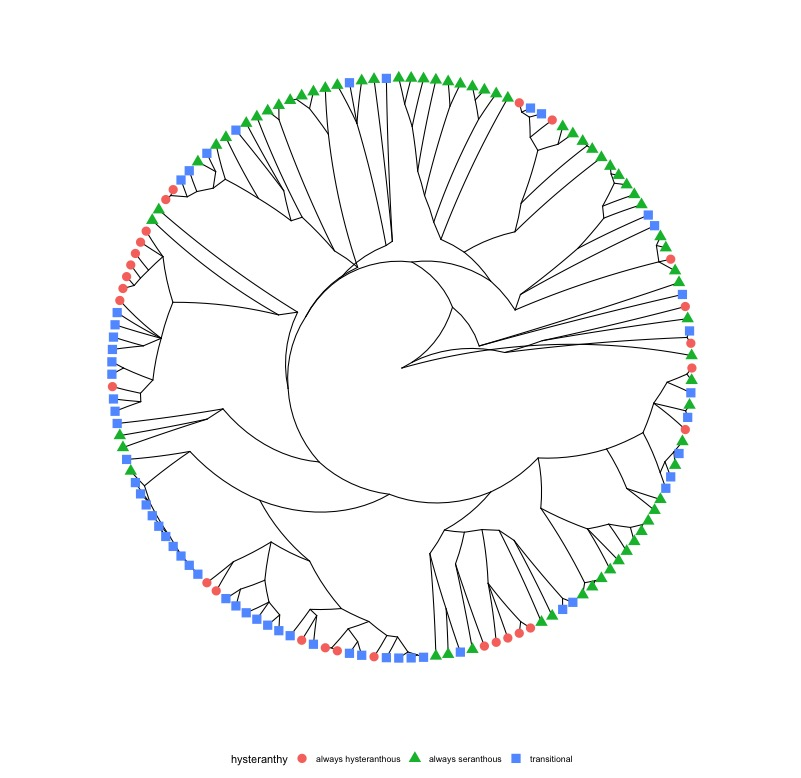
\includegraphics[height=.8\textheight]{..//figure/michtreeplot.jpeg}
    \caption{MTSV phylogeny}
    \label{fig:Figure S3}
    \end{figure}
    
     \begin{figure}
    \centering
    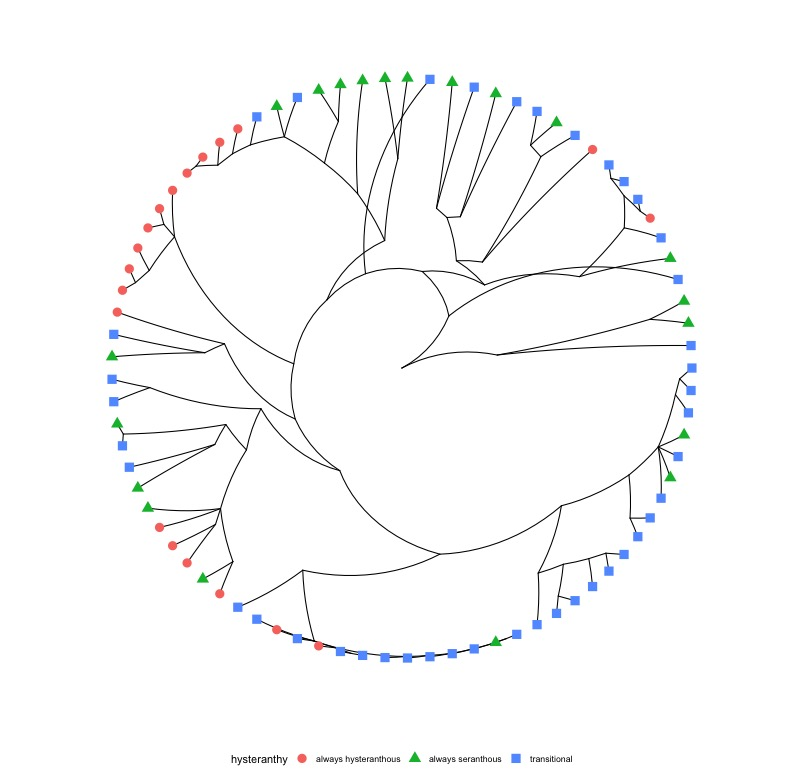
\includegraphics[height=.8\textheight]{..//figure/silvtreeplot.jpeg}
    \caption{USFS Phylogeny}
    \label{fig:Figure S4}
    \end{figure}
    
    \begin{figure}
    \centering
    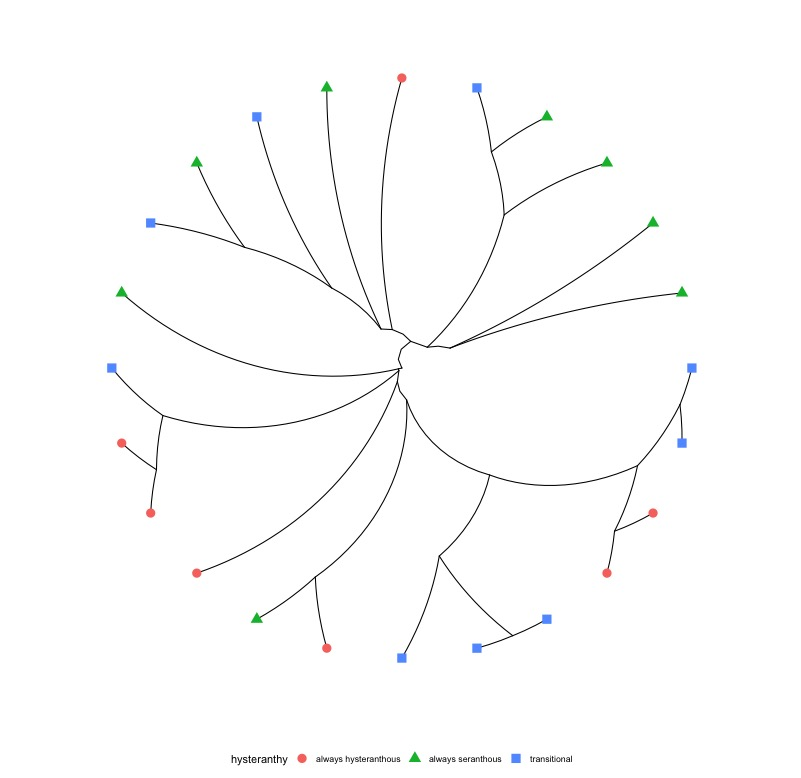
\includegraphics[height=.8\textheight]{..//figure/HFtreeplot.jpeg}
    \caption{HF Phylogeny}
    \label{fig:Figure S5}
    \end{figure}




\end{document}
